\documentclass[12pt]{article}
\usepackage[margin=1in]{geometry}
\usepackage{amsmath}
\usepackage{cancel}
\usepackage{graphicx}
\setlength{\parskip}{0.3em}
\setlength{\parindent}{0pt}
% 使用系统字体,需要 XeLaTeX 或 LuaLaTeX 编译
\usepackage{fontspec}
\setmainfont{Times New Roman}
\usepackage{xcolor}
\usepackage{float}
\newcommand{\mdavg}[2]{\langle #1 \rangle\!\langle #2 \rangle}
\newcommand{\avg}[1]{\left\langle #1 \right\rangle}
\newcommand{\doubleavg}[2]{\left\langle #1 \right\rangle\!\left\langle #2 \right\rangle}
\newcommand{\inavg}[2]{\langle #1 \rangle\! [#2]}
\newcommand{\rinavg}[2]{[#1]\!\langle #2 \rangle}
\newcommand{\aket}[1]{|#1\rangle}
\newcommand{\asqu}[1]{{\langle#1\rangle}^2}
\newcommand{\sket}[1]{|#1]}
\begin{document}

\title{Note for Scattering Amplitude Computation}
\author{Su Yingze}
\maketitle

\section{4-point case}
For the four point case $\mathcal{A}(V_2\Phi^\dagger V_1 \Phi )$, we can construct the color-ordered amplitude from the residue. First, we consider the $(+,-)$ helicity
configuration. There are two feynman diagrams contributing to the color-ordered amplitude.\\
\begin{figure}[htbp]
    \centering
    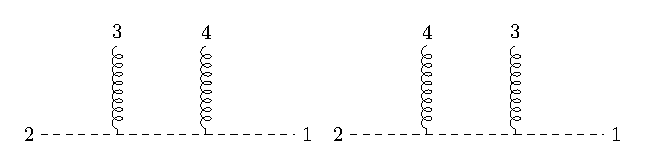
\includegraphics{4pt.eps}
    \caption{4pt.}
    \label{1}
\end{figure}

For the first diagram, the residue equals to
\begin{equation*}
    \mathcal{R}es|_{s_{12}=0}=\frac{[3 I ] [23]}{[I2]}\times \frac{\avg{I4}\avg{41}}{\avg{1I}}=\frac{\avg{24}[31]\avg{41}[23]}{[42]\avg{24}}
\end{equation*}
Similarly, the second one is
\begin{equation*}
    \mathcal{R}es|_{s_{13}=0}=\frac{\avg{4I}\avg{24}}{\avg{I2}}\times \frac{[31] [I3]}{[1I]}=\frac{\avg{24}[31]\avg{41}[23]}{\avg{32}[23]}
\end{equation*}

Then we can conclude that the four-point color-ordered amplitude $A[1,2,3^+,4^-]$ equals to
\begin{equation*}
    A[1,2,3^+,4^-]=\frac{\avg{24}[31]\avg{41}[23]}{\avg{32}[23][42]\avg{24}}=\frac{\avg{24}\avg{14}}{\avg{13}\avg{23}}
\end{equation*}

\textcolor{red}{$\star Bonus$}

It is still necessary to prove the color-ordered amplitude $A[1,2,3^+,4^+]$ equals to 0. Here we can use the color ordered Feynman rules to show the result.
\begin{equation*}
    A[1,2,3^+,4^+]\propto \frac{\left(\epsilon_3\cdot p_2\right)\left(\epsilon_4\cdot p_1\right)}{s_{23}}+\frac{\left(\epsilon_4\cdot p_2\right)\left(\epsilon_3\cdot p_1\right)}{s_{24}} 
\end{equation*}
Here we can utilize the spinor-helicity variable to express polarization vector
\begin{equation*}
    \epsilon_2^{+\mu}=\frac{\langle r_1 | \gamma^\mu | 3 ]}{\sqrt{2}\avg{r_13}},\qquad \epsilon_4^{+\mu}=\frac{\left <r_2|\gamma^\mu|4\right ]}{\sqrt{2}\avg{r_24}}
\end{equation*}
here $r_1$ and $r_2$ represent the reference spinor.

We can freely choose $r_1=r_2=1$ or 2, then $\avg{r_1 2}$,$\avg{r_2 1}$,$\avg{r_1 1}$,$\avg{r_2 2}$, two of them equal to 0, so we can conclude that
\begin{equation*}
    A[1,2,3^+,4^+]=0
\end{equation*}
\section{5-point case}
For the 5-point case, we can utilize the BCFW recursion relation which can help us generate higher point amplitude from lower point on-shell subamplitudes. Here, 
we always consider the MHV (Maximal helicity violation) amplitude. 
\par
If there is no special case, we always choose the following BCFW shift
\begin{gather*}
    \sket{\hat{2}}=\sket{2}-z\sket{3},\qquad \qquad \aket{\hat{3}}=\aket{3}+z\aket{3}\\
    \aket{\hat{2}}=\aket{2}, \qquad \sket{\hat{3}}=\sket{3}
\end{gather*}
where 2 always refers to antiscalar and 3 refers to gauge boson with + helicity.
\par
Let us begin with the simplest case $A[1,2,3_1^+,4_1^+,5_2^-]$, where the subscript represent which gauge group the particle belongs to. Because of the property 
of this kind of gauge theory, the color structure is invariant under the OPP (Order Preserving Permutation), in this case, for example,
\begin{equation*}
    (3_1^+,4_1^+,5_2^-)\qquad (3_1^+,5_2^-,4_1^+)\qquad(5_2^-,3_1^+,4_1^+)
\end{equation*}
give us the same color factor. So in the process of BCFW recursion, these three order offer the same amplitude. We can draw all diagrams contributing to the BCFW process, the first two are following
\par
\begin{figure}[H]
    \centering
    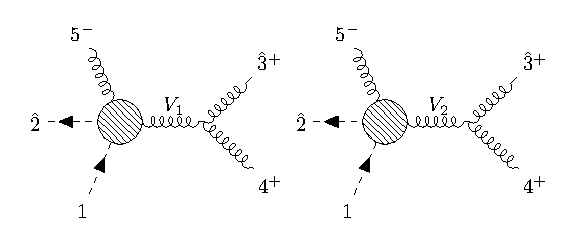
\includegraphics{5pt1.eps}
    \caption{5pt. 1}
    \label{2}
\end{figure}
It is obvious that the second diagram in Figure 2 equals to 0, because there are no interaction between the two gauge bosons.
\par
Similarly, another two diagrams equal to 0 for the same reason
\begin{figure}
    \centering
    \includegraphics{5pt2.eps}
    \caption{5pt. 2}
    \label{3}
\end{figure}
\par
The last diagram still gives 0 contribution because it includes a subamplitude $A[1,\hat{I},\hat{3}^+,4^+]=0$.
\par
\begin{figure}[H]
    \centering
    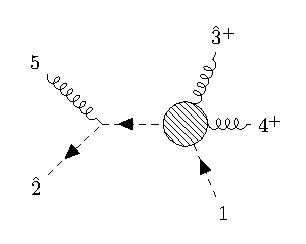
\includegraphics{5pt3.eps}
    \caption{5pt. 3}
    \label{4}
\end{figure}
Above all. only the first diagram in Figure 1 has non-vanishing contributions, so the full color ordered amplitude equals to
\begin{align*}
    A[1,2,3_1^+,4_1^+,5_2^-]&=A[1,2,\hat{I}^+,5^-]\times\frac{1}{s_{34}}\times A[\hat{3}^+,4^+,\hat{I}^-]\\
    &=\frac{\doubleavg{15}{25}}{\mdavg{1\hat{I}}{2\hat{I}}}\times\frac{1}{s_{34}}\times\frac{[\hat{3}4]^3}{[4\hat{I}][\hat{I}\hat{3}]}\\
    &=\frac{\mdavg{15}{25}\bcancel{[34]^3}}{\mdavg{14}{23}\avg{43}\bcancel{[43][43][34]}}\\
    &=\frac{\mdavg{15}{25}}{\mdavg{23}{34}\avg{41}}\\
    &=\frac{(-1)\avg{2\textcolor{green}{5}}^2\!\avg{1\textcolor{green}{5}}^2}{\textcolor{blue}{\mdavg{23}{34}\!\avg{41}}\textcolor{red}{\mdavg{25}{51}}}
\end{align*}
where we use the fact $|\hat{3}\rangle=|\hat{3}\rangle$ and following identities
\begin{equation*}
    \inavg{1\hat{I}}{\hat{I}3}=\inavg{14}{43},\quad \inavg{2\hat{I}}{\hat{I}3}=\inavg{24}{43}
\end{equation*}
and also
\begin{align*}
    \frac{[\hat{I}3]}{[4\hat{I}]}&=-\frac{\rinavg{3\hat{I}}{\hat{I}2}}{\rinavg{4\hat{I}}{\hat{I}2}}=-\frac{\rinavg{34}{42}}{\rinavg{43}{\hat{3}2}},\quad(\avg{\hat{3}2}=\avg{32}+z\avg{22}=\avg{32})\\
    &=\frac{\avg{42}}{\avg{32}}
\end{align*}
here green refers to the particle with (-) helicity, red refers to particles belong to gauge group 1, red refers to particles belong to gauge group 2.
\par
Similarly, it is very easy to obtain another color-ordered amplitude $A[1,2,3_1^+,4_1^-,5_2^+]$
\begin{align*}
    A[1,2,3_1^+,4_1^-,5_2^+]=
    \frac{(-1)\avg{2\textcolor{green}{4}}^2\!\avg{1\textcolor{green}{4}}^2}{\textcolor{blue}{\mdavg{23}{34}\!\avg{41}}\textcolor{red}{\mdavg{25}{51}}}
\end{align*}
and also $A[1,2,3_1^-,4_1^+,5_2^+]$ equals to
\begin{equation*}
    A[1,2,3_1^-,4_1^+,5_2^+]=
    \frac{(-1)\avg{2\textcolor{green}{3}}^2\!\avg{1\textcolor{green}{3}}^2}{\textcolor{blue}{\mdavg{23}{34}\!\avg{41}}\textcolor{red}{\mdavg{25}{51}}}
\end{equation*}
But here we need to emphasize that it is necessary to choose another BCFW shift, like $[1,5^+ \rangle$, as $[2,3^- \rangle$ is not a valid shift. 
\section{6-point case}
Here we consider $(V_2V_2\Phi^\dagger V_1V_1 \Phi)$ case, the corresponding color-ordered amplitude is $A[1,2,3_1^+,4_1^+,5_2^+,6_2^-]$.
Similarly, the fowwling orders all give us the same color factor
\begin{gather*}
    (3_1^+,4_1^+,5_2^+,6_2^-)\qquad(3_1^+,5_2^+,4_1^+,6_2^-)\qquad (3_1^+,5_2^+,6_2^-,4_1^+)\\
    (5_2^+,3_1^+,4_1^+,6_2^-)\qquad(5_2^+,3_1^+,6_2^-,4_1^+)\qquad (5_2^+,6_2^-,3_1^+,4_1^+)
\end{gather*}
Only two diagrams have semmingly non-zero contributaion,
\par
\begin{figure}[H]
    \centering
    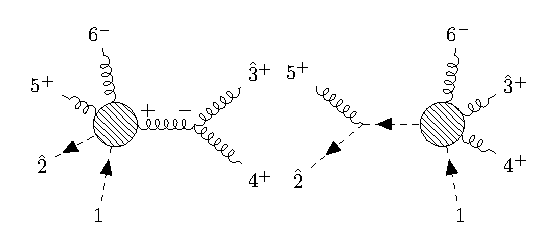
\includegraphics{6pt.eps}
    \caption{6pt.}
    \label{5}
\end{figure}
so the full color ordered amplitude equals to
\begin{align*}
    A_1&=\frac{(-1)\asqu{\hat{2}6}\asqu{16}}{\mdavg{25}{56}\!\avg{61}\!\mdavg{\hat{2}\hat{I}}{\hat{I}1}}\times\frac{1}{s_{34}}\times\frac{[\hat{3}4]^3}{[4\hat{I}][\hat{I}\hat{3}]}\\
    &=\frac{\asqu{26}\avg{16}}{\mdavg{25}{56}\!\mdavg{\hat{2}\hat{I}}{\hat{I}1}}\times\frac{1}{s_{34}}\times\frac{[34]^3}{[4\hat{I}][\hat{I}3]}\\
    &=\frac{\asqu{26}\avg{16}\bcancel{[34]^3}\bcancel{\avg{42}}}{\mdavg{25}{56}\!\mdavg{41}{32}\!\avg{43}\bcancel{[43][43][34]}\bcancel{\avg{24}}}\\
    &=\frac{\asqu{26}\!\asqu{16}}{\textcolor{blue}{\mdavg{23}{34}\!\avg{41}}\!\textcolor{red}{\mdavg{25}{56}\!\avg{51}}}
\end{align*}
where we have used the fact $\aket{\hat{2}}=\aket{2}$, $\sket{\hat{3}}=\sket{3}$, and the following identities
\begin{equation*}
    \inavg{2\hat{I}}{\hat{I}3}=\inavg{24}{43}, \qquad \rinavg{4\hat{I}}{\hat{I}1}=\rinavg{43}{\hat{3}1}
\end{equation*}
The point here is that we first $\avg{\hat{3}1}$ which does not appear in 5-point case, so we nned to compute it carefully
\begin{gather*}
    \text{pole position}: \quad \hat{P_{34}}^2=0=2P_3\cdot P_4=\inavg{4\hat{3}}{34}\qquad\Rightarrow \qquad \avg{4\hat{3}}=0\\
    \avg{43}+z\avg{42}=0\qquad \Rightarrow \qquad z=-\frac{43}{42}
\end{gather*}
then
\begin{align*}
    \avg{\hat{3}1}=\avg{31}+z\avg{21}&=\avg{31}-\frac{\avg{43}}{\avg{42}}\avg{21}\\
    &=\frac{\mdavg{42}{31}-\mdavg{43}{21}}{42}\\
    &=\frac{\mdavg{41}{32}}{\avg{42}}
\end{align*}
where we have used the Fierz identity
\begin{equation*}
    \mdavg{42}{31}+\mdavg{41}{23}+\mdavg{43}{12}=0.
\end{equation*}
Simiraly, we can compute the second diagram
\begin{equation*}
    A_2=\frac{[\hat{2}5][5\hat{I}]}{[\hat{I}\hat{2}]}\times\frac{1}{s_{25}}\times \frac{(-1)\asqu{16}\asqu{\hat{I}6}}{\mdavg{\hat{I}\hat{3}}{\hat{3}4}
    \!\mdavg{41}{\hat{I}6}\!\avg{61}}
\end{equation*}
but from the pole position
\begin{equation*}
    \hat{P_{25}}^2=0=2P_2\cdot P_5=\inavg{52}{\hat{2}5}\qquad\Rightarrow \qquad [\hat{2}5]=0,
\end{equation*}
and simiraly
\begin{equation*}
    [\hat{2}\hat{I}]=[5\hat{I}]=0.
\end{equation*}
Then we can conclude that the left part of the amplitude equals to 0 so $A_2=0$. Finally, we obtain the color-ordered amplitude 
\begin{equation*}
    A[1,2,3_1^+,4_1^+,5_2^+,6_2^-]=A_1+A_2=\frac{\asqu{26}\!\asqu{16}}{\textcolor{blue}{\mdavg{23}{34}\!\avg{41}}\!\textcolor{red}{\mdavg{25}{56}\!\avg{51}}}.
\end{equation*}
\section{n-point case}
Here, we first propose a compact formula for the color-ordered amplitude
\begin{equation*}
    A=\frac{\asqu{2a}\!\asqu{1a}}{\underbrace{\avg{2\star}\cdots \avg{\star 1}}_{SU(N_1)}\underbrace{\avg{2\ast }\cdots \avg{\ast 1}}_{SU(N_2)}}
\end{equation*}
where a refer to the particle with - helicity, whichever gauge group it belongs to. And, `$\star$' refers to the ordering for the first gauge group, `$\ast$'
refers to the ordering for the second gauge group. We suppose there are $n_1$ gauge boson 1, $n_2$ gauge boson 2, so the n-point means that $n=n_1+n_2+2$.
\par
The usual way to prove this kind of compact formula is deduction. First we suppose that all of the amplitudes with external point lower than n satisfy the compact formula.
And although there are $\frac{(n_1+n_2)!}{n_1!n_2!}$ OPP, we just need to consider some of them. 
\end{document}